\chapter{Results \& Discussion}
\section{\label{section:the_data}The AOLME Dataset}
The AOLME dataset is an enormous repository of over 900 hours of video
recordings of students. The videos contain students
interacting with facilitators, their peers and computers to write code in
Python on the Raspberry Pi.  The dataset is wealth of information but difficult
to exploit in its current state.  The data used for this thesis is a subset of
the entire AOLME dataset. By hand, we have selected several videos and extracted
typing and writing clips from the original dataset and are using these as ground
truth for measuring the accuracy of our methods.

As Figure \ref{fig:typing_writing} suggests, we are only using a cropped version
of the video. The reason for this is that we are not attempting to solve the tracking
problem in this thesis, only the classification problem. Hence, we assume that
the videos entering into our software have already been clipped and cropped with
the target activities inside of them and the corresponding lack of the activity.
Our subset of the AOLME database consists of the following:

\begin{itemize}
\item Twenty videos of typing
\item Twenty videos of no typing
\item Twenty videos of writing
\item Twenty Videos of no writing
\end{itemize}

\section{\label{section:accuracy} Accuracy of Classification}
In this section we explore how well our results are for both the classification
of typing and writing videos using the techniques described in methods chapter.

For our first set of results, we ran to classifying typing motions in videos.
The input messages into the cluster are shown in Table \ref{tab:message_list}.
The original dataset, however, contains 10-20 for each of the training classifications,
we have left them out in this table for brevity.
\begin{table}[h]

  \begin{tabular}{ | l | l | l | p{2cm} |}
  \hline
  \textbf{path} & \textbf{classification} & \textbf{sqs\_queue} & \textbf{algorithm}\\ \hline
  aolme/data/typing/seg\_1.mp4 & 1 & feature\_queue & farneback \\\hline
  aolme/data/typing/seg\_2.mp4 & 1 & feature\_queue & farneback \\\hline
  aolme/data/typing/seg\_3.mp4 & 1 & feature\_queue & farneback\\\hline
  aolme/data/typing/seg\_4.mp4 & 1 & feature\_queue & farneback\\\hline
  aolme/data/typing/seg\_5.mp4 & 1 & feature\_queue & farneback\\\hline
  aolme/data/typing/seg\_6.mp4 & 1 & feature\_queue & farneback\\\hline
  aolme/data/typing/seg\_7.mp4 & 1 & feature\_queue & farneback\\\hline
  aolme/data/typing/seg\_8.mp4 & 1 & feature\_queue & farneback\\\hline
  aolme/data/typing/seg\_9.mp4 & 1 & feature\_queue & farneback\\\hline
  aolme/data/typing/seg\_10.mp4 & 1 & feature\_queue & farneback\\\hline
  \ldots & \ldots & \ldots & \ldots\\\hline
  aolme/data/notyping/seg\_1.mp4 & 2 & feature\_queue & farneback\\\hline
  aolme/data/notyping/seg\_2.mp4 & 2 & feature\_queue & farneback\\\hline
  aolme/data/notyping/seg\_3.mp4 & 2 & feature\_queue & farneback\\\hline
  aolme/data/notyping/seg\_4.mp4 & 2 & feature\_queue & farneback\\\hline
  aolme/data/notyping/seg\_5.mp4 & 2 & feature\_queue & farneback\\\hline
  aolme/data/notyping/seg\_6.mp4 & 2 & feature\_queue & farneback\\\hline
  aolme/data/notyping/seg\_7.mp4 & 2 & feature\_queue & farneback\\\hline
  aolme/data/notyping/seg\_8.mp4 & 2 & feature\_queue & farneback\\\hline
  aolme/data/notyping/seg\_9.mp4 & 2 & feature\_queue & farneback\\\hline
  aolme/data/notyping/seg\_10.mp4 & 2 & feature\_queue & farneback\\\hline
  \end{tabular}
  \caption{Data that is sent to the SQS for calculation on the cluster. The
  original dataset includes 10-20 for both classifications}
  \label{tab:message_list}
\end{table}

Using our R code, we then plot some statistics about the vectors that have come
back from the cluster.
% The first column represents the statistics from videos that have the activity
% in them, and the second column represents the lack of that activity. Just from
% visual inspection, we can already see that there differences in the overall
% statistics, which means that we should have very good luck with our support
% vector machine properly classifying the results.

\FloatBarrier

% \begin{figure}[h]
%   \label{fig:typing_box_whiskers}
%   \centering
%   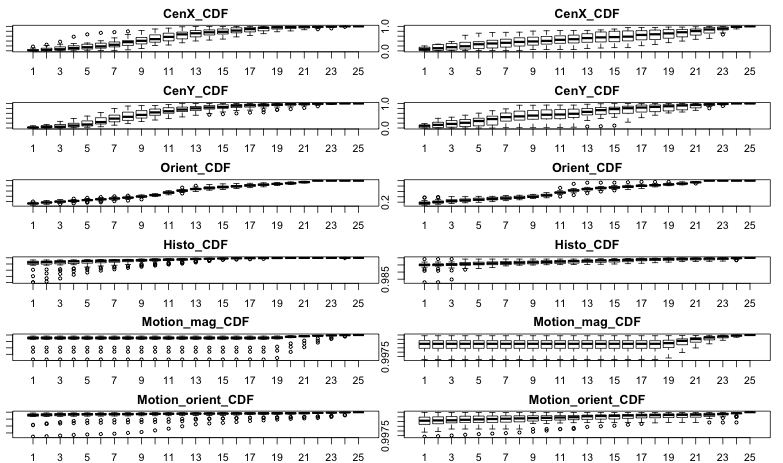
\includegraphics[width=\textwidth]{figures/typing_box_whiskers}
%   \caption{Box and whiskers plot of CDFs for typing. The first column represents the
%   statistics for typing and the second column represents the statistics for no
%   writing.}
% \end{figure}

With those feature vectors, we found that we were able to get the confusion matrix
shown in Table \ref{tab:typing_confusion}
\begin{table}[h]
  \begin{centering}
  \begin{tabular}{| l | l | l |}
  \hline
   & \textbf{typing} & \textbf{no typing}\\ \hline
  \textbf{typing} & 19 & 1 \\ \hline
  \textbf{no typing} & 3 & 17 \\ \hline
  \end{tabular}
  \caption{Confusion matrix for classification accuracy for typing}
  \label{tab:typing_confusion}
\end{centering}
\end{table}

\FloatBarrier

From Table \ref{tab:typing_confusion} we can see that we get 90\% accuracy for
classifying typing motions on the keyboard. We had difficulty classifying
videos that had significant motion in them, but the motion was not typing and
we also found that we had trouble classifying the videos where there is was
not much typing in the videos that were classified as typing. But overall, when the
scene clearly had typing and when it clearly did not, we found that we had
90\% accuracy.

Our results for determining writing, however, were not as good as our results
for classifying typing. Our CDFs for typing are shown in figure

% \begin{figure}[h]
%   \label{fig:typing_box_whiskers_1}
%   \centering
%   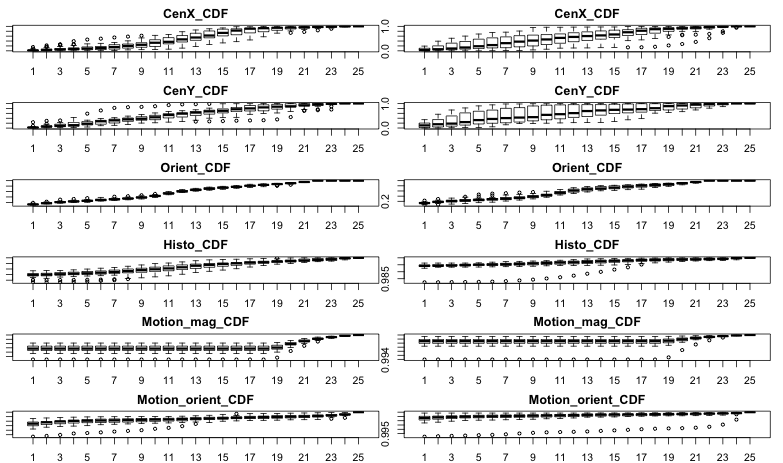
\includegraphics[width=\textwidth]{figures/writing_cdfs}
%   \caption{Box and whiskers plot of CDFs for writing. The first column represents the
%   statistics for typing and the second column represents the statistics for no
%   writing.}
% \end{figure}

\FloatBarrier

\begin{table}[h]
  \begin{centering}
  \begin{tabular}{| l | l | l |}
  \hline
   & \textbf{writing} & \textbf{no writing}\\ \hline
  \textbf{writing} & 18 & 2 \\ \hline
  \textbf{no writing} & 11 & 9 \\ \hline
  \end{tabular}
  \caption{Confusion matrix for classification accuracy for typing}
  \label{tab:writing_confusion}
\end{centering}
\end{table}

As can be seen in Table \ref{tab:writing_confusion}, we did not get as good
as results for writing, only about 65\% classification. In these results we
find that our algorithm struggled more with classifying videos that had no
writing in them as having writing in them. This may mean that the motion vectors
we are extracting are highly dependent on the type of scene we are looking at. Furthermore,
the original algorithm was developed in Matlab and then ported to C++ for this thesis. We
saw differences in the feature vectors between the two implementations; however,
classification results proved to be very similar.

\section{\label{section:scalability}Proof of Scalability}
In order to show that our system is scalable, we record the time it takes for
the cluster to perform certain repetitive tasks. For the first experiment, we
have the cluster operate using only a single EC2 instance, and then scale the
experiment by one instance and compare how long it takes to calculate 10 2.1MB
videos. For this experiment, we used Amazon's t2.micro instance which contains 1
virtual CPU running on a high frequency Intel Xeon processor with turbo up to
3.3GHz and contains 1GB of memory. Because t2 instances are designed to  have
burstable performance, Amazon does not list any specific processor on their webpage
as can be seen in Figure \ref{fig:instance_table}. Amazon designed
these instances like this so that the user is not consistently charged  for using
high performance CPUS, but rather only when they need the performance are  they
charged for those compute cycles. As a result, T2 instances can take
advantage of Intel capabilities such as native instructions for AES
encryption (AES-NI) Advanced Vector Extensions (AVX) for floating point and
Turbo Boost where the CPU core can be made to run faster. So for this reason, we
cannot give an exact chip type that was used when performing these computations
because it is possible that the virtual CPU that we were initially assigned, is
not the same CPU that we received later on in the experiment. This is the
instance that is considered to be part of the free tier program. Our instance
runs a special Amazon Machine image The results from this experiment are show in
Figure
\ref{fig:speed_up}

\begin{figure}[h]
  \label{fig:instance_table}
  \centering
  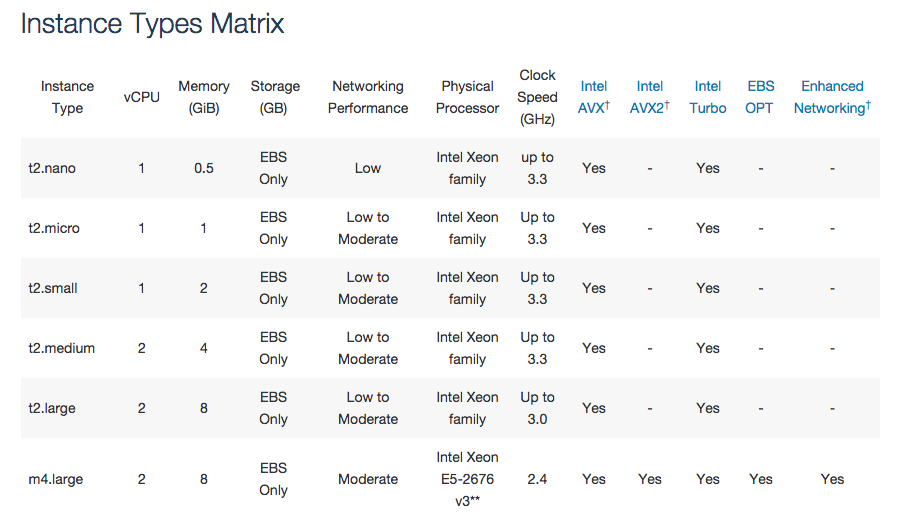
\includegraphics[width=\textwidth]{figures/instance_table}
  \caption{A subset of instances that can be used for processing on the cloud.
  Notice how t2 instances are not associated with any specific processor, only
  the processor family.}
\end{figure}

\begin{figure}[h]
  \label{fig:speed_up}
  \centering
  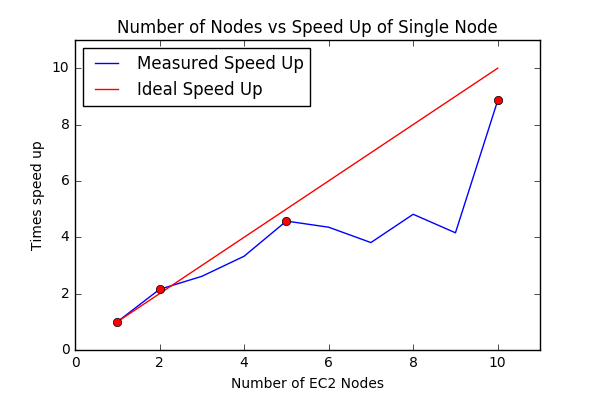
\includegraphics[width=.8\textwidth]{figures/speed_up}
  \caption{Leaving the number of videos to process the same, we increase the
  number of EC2 instances to illustrate the speed up.}
\end{figure}

From Figure \ref{fig:speed_up}, we can see that as long as the number of instances
that we have divides evenly into the number of videos that calculate, then we
get a linear increase in speed. In other words, we get 10x speed up when using
10 instances rather than just using a single instance.

The size of the videos does matter. The smaller that the videos are, the less
the overhead is when running the cluster. The reason for this is because not only
does it take longer to transfer larger videos, but it also takes more time to process
them. So from our experiments, it looks like keeping the videos under 2MB is optimal
for distributing and processing the videos.
We tested how well the t2.micro instances performed against our MacBook Pro 15 inch
with an Intel Core i7 clocked at 2.7 GHz and has 16GB of RAM. It should also be
noted that the Macbook Pro contains an AMD Radeon R9 M370X GPU with 2048 GB of
memory. This allows us to take advantage of the TAPI programming model that
we leverage as described in the Methods section.  As shown in figure \ref{fig:size_matters},
we can see that even though we have significant processing power locally, we still
must receive the message from the queue and then process the videos; therefore
there is actually little gained in terms of performance even though we are able
to leverage the onboard GPUs. Figure \ref{fig:size_matters} also demonstrates
that 10 instances run at exactly the same speed as a single instance. So from this
graph we can also infer that even though we have a higher power CPU technically
on the t2.micro instance, we are able to leverage OpenCV's transparent API and
take advantage of the local GPU on the Macbook Pro.


\begin{figure}[h]
  \centering
  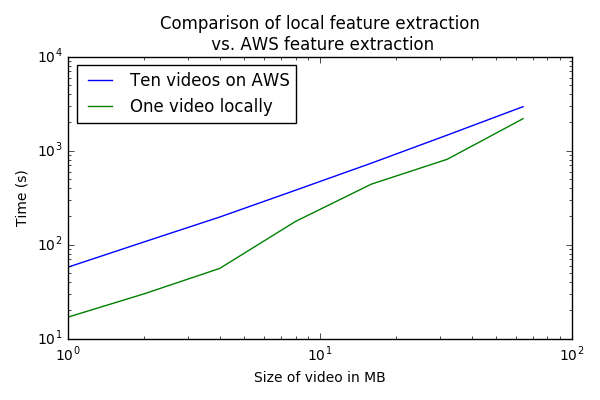
\includegraphics[width=.9\textwidth]{figures/aws_vs_local.png}
  \caption{Comparison of the time it takes for a single node to process 1 video
  vs the time it takes a cluster to process 10 videos. Videos vary in size to
  test the efficacy of choosing to send smaller vs larger videos to the cluster.
  A single t2.mirco instance was included to show that a single instance takes
  just as long as 10 instances.}
  \label{fig:size_matters}
\end{figure}

\FloatBarrier

Additionally, we can see that the performance of S3 has a linear download and upload
speed from an EC2 instance. We have collected data that calculates the mean of 10
sample download-upload pairs of a given file size. The results of this are shown
in Figures \ref{fig:s3_upload_speed} and \ref{fig:s3_download_speed}. So as expected,
we can rely on S3 to give us a linearly predictable download and upload rate.
Because though, it can take a significant time to download, process, and upload videos,
it is more beneficial for the distributed system to break videos into smaller
pieces so that no one node is occupied for a long period of time. If this
notion is followed, it is much easier to scale the feature extractions horizontally.

\begin{figure}[h]
  \centering
  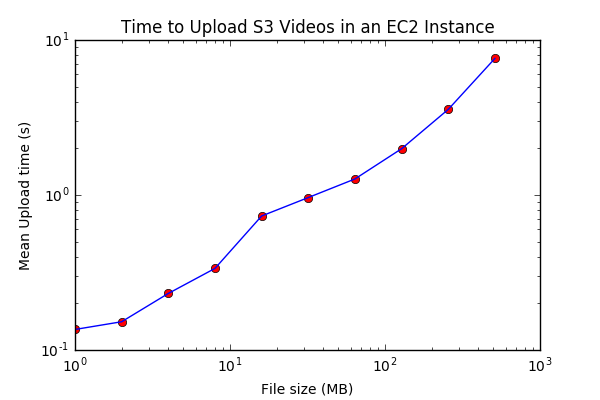
\includegraphics[width=.8\textwidth]{figures/s3_upload_speed}
  \caption{Average time to upload varying file sizes in S3 using an EC2 instance. }
  \label{fig:s3_upload_speed}
\end{figure}


The upload times can be seen in Table \ref{tab:upload_speed}
\begin{table}[h]
  \begin{tabular}{lr}
\toprule
{File Size} &         Seconds \\
\midrule
Upload 1MB (s)   &  0.135685 \\
Upload 2MB (s)   &  0.152184 \\
Upload 4MB (s)   &  0.231676 \\
Upload 8MB (s)   &  0.336037 \\
Upload 16MB (s)  &  0.732164 \\
Upload 32MB (s)  &  0.963004 \\
Upload 64MB (s)  &  1.269231 \\
Upload 128MB (s) &  1.989168 \\
Upload 256MB (s) &  3.567965 \\
Upload 512MB (s) &  7.608010 \\
\bottomrule
\end{tabular}
\caption{Average upload speeds in seconds on an EC2 instance to an S3 bucket}
\label{tab:upload_speed}
\end{table}


\begin{figure}[h]
  \centering
  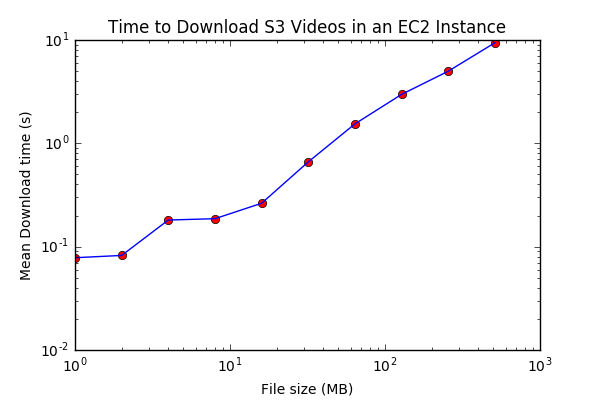
\includegraphics[width=.8\textwidth]{figures/s3_download_speed}
  \caption{Average time to download varying file sizes in S3 using an EC2 instance. }
  \label{fig:s3_download_speed}
\end{figure}

The download times can be seen in Table \ref{tab:download_speed}
\begin{table}[h]
  \begin{tabular}{lr}
  \toprule
  {File Size} &         Seconds \\
  \midrule
  Download 1MB (s)   &  0.078182 \\
  Download 2MB (s)   &  0.082242 \\
  Download 4MB (s)   &  0.181033 \\
  Download 8MB (s)   &  0.186510 \\
  Download 16MB (s)  &  0.263108 \\
  Download 32MB (s)  &  0.661547 \\
  Download 64MB (s)  &  1.542783 \\
  Download 128MB (s) &  2.976941 \\
  Download 256MB (s) &  4.990264 \\
  Download 512MB (s) &  9.406564 \\
  \bottomrule
  \end{tabular}
\caption{Average Download speeds in seconds on an EC2 instance from S3}
\label{tab:download_speed}
\end{table}


When we consolidate the numbers above, we find that we end up with an average
upload speed of 37.0486495118 MB/s and an average download speed of 40.149124154 MB/s.

\FloatBarrier

\section{Discussion}
In the previous sections we showed that we can accurately classify typing in
small segments of video and demonstrated how to we can horizontally and vertically
scale our system in the cloud. In order to achieve this, we had to find the
optimal points to break the system apart so that the computationally
expensive aspects of the system could be handled by the compute cluster, and the
quick computations could be handled by the master node, or a client node.
The quick computations in the master or client node are made possible by the
cluster of computers reducing the video files down to only a few significant
CDFs. Thus, given a set of CDFs that are only tens of kilobytes in size, we
were able to quickly train a machine learning algorithm using some ground truth
videos, and then could quickly classify features being output from the system
in microseconds.

Based on the plot in Figure \ref{fig:speed_up}, we showed that the system
we have proposed in this thesis is horizontally scalable to at least 10 nodes.
More nodes could have easily been selected, but in an attempt to keep the cost
of this thesis low, we decided to only use what is available by default in the
AWS cloud. However, based on the success of other applications, such as
Netflix that have used cloud technologies to scale their system to hundreds
or even thousands of nodes, there is no reason to believe that this system
would not scale to the same order of magnitude, though more care would probably
need to be taken to scale the nodes strategically on the AWS network services.

Finally we showed that is possible to create a greatly reduced feature space
from videos and accurately classify when students are typing at nearly 90\%.
Because the feature space is so significantly reduced after processing the
videos on the cloud, classification of videos becomes a task that takes only
milliseconds once the system has been trained. Furthermore, even training, once
the feature space has been reduced, only takes a matter of minutes for very
large datasets. As we also showed, we did not get very statistically significant
results for classifying writing. It is unclear why the motion vectors for this
activity were not as significant as they were for typing.

\subsection{Limitations}
One of the limitations of this research was retrieving sufficient ground truth
data for the videos that are analyzed. Many of the datasets that were
used in other research in this area have large datasets with ground truth
associated with them. Since the dataset we use in this paper is novel, we didn't
have the time nor the resources to generate a dataset with hundreds of samples
with ground truth.

Additionally, we were resource bound financially for this research. If we had more
money to conduct the research, we could have tested the system at a larger
scale to prove that it would work beyond just ten nodes.

Since most of the focus on this paper is primarily to investigate how to
efficiently distribute and analyze videos in the AWS cloud, there was less time
for investigation in determining the best ways to classify the human activity.
One of the short comings of this research was that it didn't address trying to
classify typing against writing. In other words, the paper doesn't investigate
classification of typing from writing, it only investigates whether we classify
a video as having typing in it, or not having typing in it.



 % But this is by no means a full implementation of the system
 % we would like to create for interactive analysis of AOLME videos. Figure
 % \ref{fig:full_system}
 %
 % \begin{figure}[h]
 %   \label{fig:full_system}
 %   \centering
 %   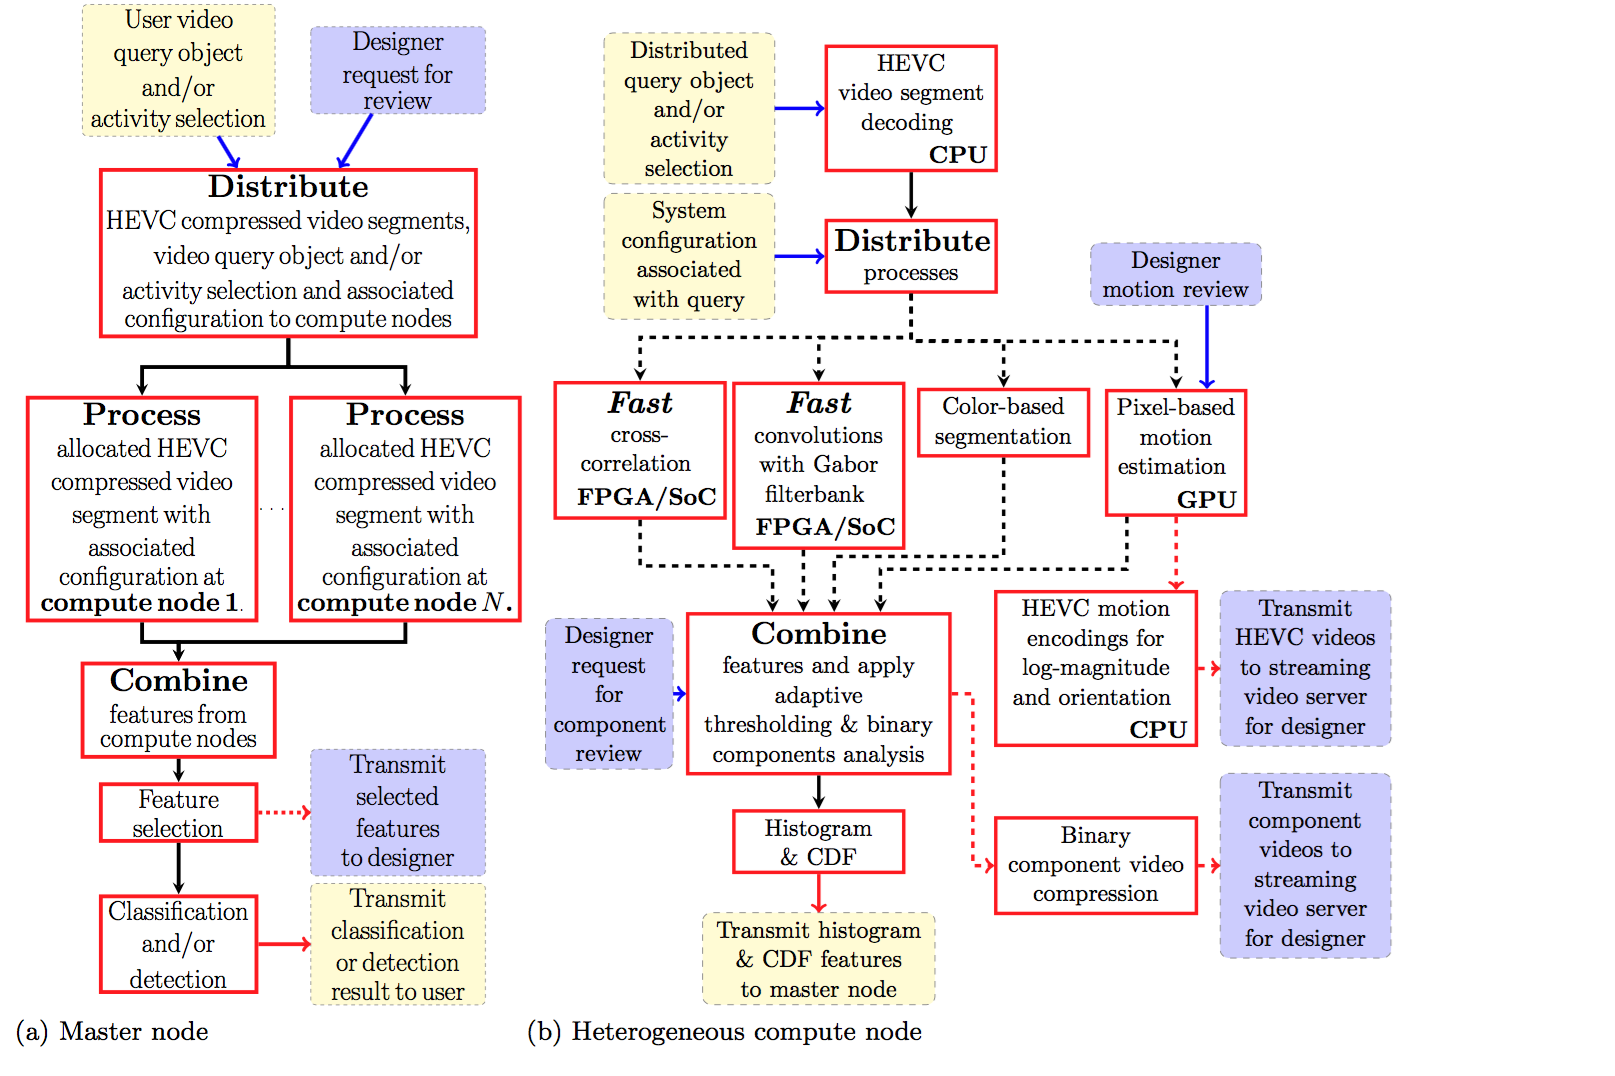
\includegraphics[width=\textwidth]{figures/full_system}
 %   \caption{Illustration of the end goal of the VIDA system. (a) shows the
 %   functions of the master node, and (b) shows the functions of the slave node.
 %   For this thesis we have implemented parts of the distribution as well as parts
 %   of the compute node.}
 % \end{figure}
 %
 % \FloatBarrier

 % For this thesis we have essentially shown that it is possible to distribute
 % small parts of the video from the master node to be consumed by the compute nodes
 % and then combined into the CDF features. We have not made the work that we have
 % done in this thesis interactive yet, but future work should be able to leverage
 % what we have done in this thesis to do so. In order to achieve the interactive
 % system that is shown in Figure \ref{fig:full_system}, we would need the master
 % node to break the HEVC videos into small 1-2MB segments to send out to the compute
 % cluster and then have the video results recombined into a single feature vector
 % when the results are collected again back at the master. This modification is
 % imperative to ensure that each one of the compute nodes can handle the workload
 % in a timely fashion. It could mean the difference between hours and minutes
 % as illustrated in Figure \ref{fig:size_matters}.
